\documentclass[11pt]{article}
\usepackage{amsmath}
\usepackage{amssymb}
\usepackage{amsthm}
\usepackage{caption}
\usepackage{cleveref}
\usepackage{enumitem}
\usepackage{graphicx}
\usepackage[totalwidth=480pt, totalheight=680pt]{geometry}
\usepackage{mathrsfs}
\usepackage{tikz}

\captionsetup{width=0.8\textwidth}
\DeclareMathOperator*{\argmax}{arg\,max}
\newtheorem{definition}{Definition}
\newtheorem{lemma}{Lemma}
\newtheorem{theorem}{Theorem}
\setlength{\tabcolsep}{1em}
\setlist{listparindent=\parindent, parsep=0pt}

\newcommand{\EE}{\mathbb{E}}
\newcommand{\PP}{\mathbb{P}}
\newcommand{\RR}{\mathbb{R}}

\begin{document}

\title{Rank verification for exponential families}
\author{Kenneth Hung \and William Fithian}
\date{\today}
\maketitle

\begin{abstract}
This paper deals with the selective inference problem encountered in rank verification --- verifying the order of the natural parameters in exponential families. We constructed a selective level-$\alpha$ test for verifying the largest natural parameter, which provides familywise error rate (FWER) and false discovery rate (FDR) control as we extend it into a step-down procedure. We also provide selective confidence bound for the difference between the largest and the second largest natural parameters.
\end{abstract}

\section{Introduction}
\label{sec:introduction}

We often make observations that form a joint exponential family distribution. While it might be relatively obvious in the independent case, the observations can well be dependent and hinge on the natural parameters. Comparison of these natural parameters can produce useful inferences.

A classic question is on how to statistically verify empirical rankings based on simple exponential family models. As motivation, consider a 2016 Quinnipiac University poll of $890$ Iowa Republicans Poll. \cite{quinnipiac} The poll found that Trump was in the lead with $31\%$ of the vote, Cruz is the first runner-up with $24\%$, followed by Rubio at $17\%$. The other ten candidates, including ``Don't know'', trailed behind. \Cref{tbl:poll} shows the results of the poll. Note that we have made a simplifying assumption that poll represents a random sample of Iowa Republicans --- i.e.\ that the data are multinomial, with parameter $\left(\pi_{\text{Trump}}, \pi_{\text{Cruz}}, \pi_{\text{Rubio}}, \ldots\right)$ representing their support in the Iowa Republican population. In reality, Quinnipiac University Poll Institute has processed the data to make the sample more representative of the population of likely voters.

\begin{table}[htbp]
\begin{center}
\begin{tabular}{c c c c}
	\hline
	Rank & Candidate & Result & Votes \\
	\hline
	$1$ * & Trump & $31\%$ & $276$ \\
	$2$ * & Cruz & $24\%$ & $214$ \\
	$3$ * & Rubio & $17\%$ & $151$ \\
	$4$ * & Carson & $8\%$ & $71$ \\
	$5$ & Paul & $4\%$ & $36$ \\
	$6$ & Bush & $4\%$ & $36$ \\
	$7$ & Huckabee & $3\%$ & $27$ \\
	$\vdots$ & $\vdots$ & $\vdots $ & $\vdots$ \\
	\hline
\end{tabular}
\end{center}
\caption{Results from a February 1, 2016 Quinnipiac University poll of $890$ Iowa Republicans. To compute the last column (Votes), we make the simplifying assumption that the reported percentages in the third column (Result) correspond to raw vote shares among survey respondents. The asterisks indicate that the rank is verified through a step-down procedure.}
\label{tbl:poll}
\end{table}

Having observed that Trump received the most votes in this poll, we want to ask whether he is actually in the lead in the population of all Iowa Republicans. Intuitively, we would compare Trump to Cruz, as well as the other candidate. This intuitive method however has a few issues.

\begin{enumerate}

\item This has a hidden upward selection bias, or ``winner's curse'', as we are only testing this hypothesis as Trump is leading in the polls. In other words, the hypothesis itself is random. Alternatively, we can note that the marginal type I error rate is indeed not so straightfoward. If the null hypothesis is ``$H_0: \text{Leader in polls has most support}$'', then for any distribution $F$ the marginal type I error rate is

\begin{equation}
\PP_F\left(\text{reject } H_0\right) = \sum_{j \text{ is a candidate}} \PP_F\left(\text{reject } H_0 \middle| j \text{ leads in polls}\right) \PP_F \left(j \text{ leads in polls}\right).
\label{eqn:marginal_error}
\end{equation}

\item Comparing Trump to all other candidates involves multiple comparisons. Without considering the structure of this problem, common methods like Tukey's correction \cite{Tukey:1951} may largely decrease the test power.

\end{enumerate}

We will construct a test as outlined by Fithian, Sun and Taylor in \cite{Fithian:2014ws}. The fundamental idea is to consider the selective type I error rate
$$\PP_F\left(\text{reject } H_0 \middle| j \text{ leads in polls} \right), ~~~~~~~~ \text{where $j$ is a candidate,}$$
instead. Note that controlling this selective type I error rate at $\alpha$ provides control of the marginal type I error rate given in \Cref{eqn:marginal_error} at $\alpha$ too.

Surprisingly, this also tackles the second issue above. The test reduces the multiple comparison problem into one comparison between Trump and Cruz. In fact, if 100 John Does entered the race with practically no support from the Iowa Republicans, the change in number of candidates will not change the test.

More generally, when we observe a random vector $(X_1, \ldots, X_n)$ from an exponential family, and whichever random variable is largest, we want to test whether it is in fact stochastically larger than the other random variables.

\subsection{Related work}

Gutmann and Maymin \cite{Gutmann:1987fk} has worked on a similar question where the observations are from a location family, and the location parameters are compared. In contrast, a related paper by Karnnan and Panchapakesan \cite{Karnnan:2009iv} discussed a scale family instead, comparing the scale parameters. Bofinger \cite{Bofinger:1991hv} gave a location-scale family generated by the exponential distribution as well. However, as location-scale families have limited overlap with exponential families, the counterpart question for exponential families have remained unaddressed. Location-scale families assumed independence between observations, while this is not required in exponential families. A follow-up paper by Maymin and Gutmann \cite{Maymin:1992fz} gave a slightly more general result, applicable to more than location-scale families, yet still under the constraints of independence.

In the vicinity of the polling problem above, Nettleton \cite{Nettleton:2009ht} provided an asymptotic test for multinomial distribution, imposing the selection by considering intersection-union tests. Ng and Panchapakesan \cite{Ng:2007cn} also analyzed the multinomial case for an exact test, but with an additional restriction that maximum observation is a known constant.

The subset selection problem solved in \cite{Gupta:1967wg} by Gupta and Nagel can indeed be used to solve the multinomial case. They selected a subset that contains the largest, or ``tagged'', parameter with probability $1-\alpha$. Confirming the largest parameter is thus equivalent to asserting the selected subset has size $1$. \Cref{sec:multinomial_example} includes a comparison of our proposed test and their test.

\subsection{Main result}

In this paper, we focus on Schur-concave exponential family, a broad class of distribution that is defined in \Cref{sec:exponential_families} and includes various examples listed in \Cref{sec:applications}. We constructed a selective level-$\alpha$ test for verifying that the largest observation is stochastically largest as well. The test provides selective type I error control, as well as enables us to construct confidence bound on the differences between the natural parameters and verify the order of the rest of natural parameters.

\subsection{Outline}

\Cref{sec:multinomial_example} gives an exploratory example based on the multinomial distribution, along with a comparison to an earlier method by Gupta and Nagel. \Cref{sec:exponential_families} gives an in-depth discussion and proof of the main result. \Cref{sec:selective_confidence_bound,sec:step_down_procedure} extend the main result to construct confidence bounds for the gap between natural parameters and a step-down procedure that verifies the order of the rest of the natural parameters with FWER and FDR control, respectively. \Cref{sec:applications} provides a few applications, including both distributions with known tests and those without.

\section{Multinomial example}
\label{sec:multinomial_example}

Suppose we observe
$$\left(X_1, \ldots, X_n\right) \sim \text{Multinomial}\left(N, \pi\right)$$
and we want to test
$$H_{0j}: \pi_j \le \max_{k \ne j} \pi_k = \bigcup_{k \ne j} H_{0jk}: \pi_j \le \pi_k$$
when $X_j$ is larger than all other $X_k$. To break ties, we introduce independent auxiliary random variable $U_j \sim U\left[0,1\right]$, and opt to test $H_{0j}$ in the event of
$$A_j = \left\{X_j + U_j > \max_{k \ne j} X_k + U_k\right\}.$$
The distribution, written in an exponential family format, is
$$\exp\left(X_1 \log \pi_1 + \cdots + X_n \log \pi_n\right) \frac{1_{X_1 + \cdots + X_n = N}}{X_1! \cdots X_n!}.$$

Without loss of generality, we will assume $X_1$ is considered largest with the tie-breaking method above in mind. Following the construction in \cite{Fithian:2014ws}, if we want to construct $p$-values $p_{1j}$ for $H_{01j}$, we need to first re-parametrize such that the selection event $A_1$ can be expressed as the sufficient statistic. The distribution is now
$$\exp\left(\frac{X_1 - X_j}{2} \left(\log \pi_1 - \log \pi_j\right) + \cdots + \frac{X_1 + X_j}{2} \left(\log \pi_1 + \log \pi_j\right) + \cdots + X_n\right) \frac{1_{X_1 + \cdots + X_n \log \pi_n = N}}{X_1! \cdots X_n!}.$$

Next we condition on the sufficient statistics that are multiplied to the the nuisance parameter, in other words, we consider the conditional law
$$\mathcal{L}_{\pi_1 = \pi_j}\left(\frac{X_1 - X_j}{2} \middle| X_2, \ldots, \frac{X_1 + X_j}{2}, \ldots, X_n, A_1\right),$$
or equivalently, the conditional law
$$\mathcal{L}_{\pi_1 = \pi_j}\left(X_1 \middle| X_2, \ldots, \frac{X_1 + X_j}{2}, \ldots, X_n, A_1\right),$$
which is the distribution $\text{Binomial}\left(X_1 + X_j, \frac{1}{2}\right)$ truncated by the event $A_1$. The one-sided $p$-value $p_{1j}$ is thus given as
$$\frac{\sum_{t = X_1}^{X_1 + X_j} \binom{X_1 + X_j}{t} \left(\frac{1}{2}\right)^{X_1 + X_j}}{\sum_{t = \left(X_1 + X_j\right)/2}^{X_1 + X_j} \binom{X_1 + X_j}{t} \left(\frac{1}{2}\right)^{X_1 + X_j}} = \frac{\sum_{t = X_1}^{X_1 + X_j} \binom{X_1 + X_j}{t}}{\sum_{t = \left(X_1 + X_j\right)/2}^{X_1 + X_j} \binom{X_1 + X_j}{t}},$$
and to account for the tie-breaking we adopted earlier, we
\begin{itemize}
\item multiply the first term in the numerator and the numerator by $1/m$ where $m$ is the number of observations tied for largest; otherwise,
\item multiply the first term in the denominator by $1/2$ if $X_1$ and $X_2$ has the same parity.
\end{itemize}
Noticing that if there are ties for the largest the $p$-value is $1$ and the denominator is really $1/2$ otherwise, we can write
$$p_{1j} = 1 \wedge 2 \sum_{t=X_1}^{X_1 + X_j} \binom{X_i + X_j}{t}.$$

It is possible to check that $p_{12} \ge p_{1j}$ for any $j > 2$. Since the null hypothesis we are testing is a union of these smaller null hypothesis, the type I error rate is
$$\PP_{H_{01}}\left(p_{12} < \alpha \middle| A_1\right) \le \max_{j>1} \PP_{H_{01j}}\left(p_{12} < \alpha \middle| A_1\right) \le \max_{j>1} \PP_{H_{01j}}\left(p_{1j} < \alpha \middle| A_1\right) \le \alpha,$$
meaning that it is sufficient to construct a one-sided test between $X_1$ and $X_2$ and consider only $p_{12}$.

It may appear quite surprising that ``verifying a winner'' as we propose in this section requires no adjustment for multiplicity, in the sense that we only need to compare the winner to the runner- up, just as we would have done if $n = 2$. After all, we know that the winner suffer’s from a winner's curse: given $X_5$ is the winner, $X_5 / N$ would overestimate $\pi_5$, and the larger $n$ is, the more severe this bias is likely to be. However, if $X_9$ is the runner-up, then $X_9 / N$ is likely biased upward nearly as much as $X_5$. Informally, we might say that $X_9$ suffer’s from a “runner-up’s curse” that is nearly as bad as the winner's curse; as a result, $X_5 - X_9$ is actually not all that biased upward. By multiplying the $p$-value by $2$, or equivalently performing a two-tailed test, takes care of what little bias there is. Indeed, performing a two-tailed test can be viewed as a sort of ``correction for multiplicity'', albeit one that we would have to make even if $n = 2$.

\subsection{Connection with the subset selection problem}
\label{sec:compare_subset}

Gupta and Nagel \cite{Gupta:1967wg} devised a rule to select a subset that includes the maximum $\pi_j$. In other words, if the selected subset is $J\left(X\right)$, they guaranteed
$$\PP\left(\argmax_j \pi_j \in J\left(X\right)\right) \ge 1 - \alpha.$$
This was achieved by finding an integer $D$, as a function on $N$ and $n$, and select by
$$J\left(X\right) = \left\{j: X_j \ge \max_k X_k - D\right\}.$$
Gupta and Nagel also provided the method to choose $D$, which we implemented. 

\Cref{fig:power} gives the power curves for $\text{Multinomial}\left(N, \pi\right)$ and
$$\pi \propto \left(e^\delta, 1, \ldots, 1\right),$$
for various combinations of $N$ and $n$. The procedure by Gupta and Nagel coincides with our procedure at $n = 2$ if we half our $\alpha$. However as $n$ grows, the selective test shoes significantly more power than Gupta and Nagel's test even for the same $\alpha$.

\begin{figure}[htbp]
\begin{center}
\includegraphics[width = \textwidth, trim = {1.3in 0.7in 1.6in 0.6in}, clip]{plotMultinomialPower}
\end{center}
\caption{Power curves as a function of $\delta$. The plots in the first row all have $N = 50$ and the second row $N = 250$. The solid line is the power for the selective test and the dashed line Gupta and Nagel's test.}
\label{fig:power}
\end{figure}

\section{Exponential families}
\label{sec:exponential_families}

We would like to extend the result from multinomials to exponential families. We henceforth focus on exponential distribution taking the form
\begin{equation}
X \sim \exp\left(\theta_1 X_1 + \cdots + \theta_n X_n\right) g\left(X\right) h\left(\theta\right).
\label{eqn:exp_family}
\end{equation}
It is reasonable to assume that the distribution is ``symmetric'', i.e.\ if $\theta_j = \theta_k$, then the probability distribution remains the same when $X_j$ and $X_k$ are swapped. This corresponds to requiring $g\left(X\right)$ to be symmetric. We would also like to introduce a fairly mild additional condition that $g$ is {\em Schur-concave}. But first we define the notion of {\em majorization}.

\begin{definition}
For two vectors $a$ and $b$ in $\RR^n$, suppose permuting the two vectors in descending order gives
$a_{\left(1\right)} \ge \cdots \ge a_{\left(n\right)}$ and $b_{\left(1\right)} \ge \cdots \ge b_{\left(n\right)}$. We say that $a \succeq b$ ($a$ majorizes $b$) if for $1 \le i < n$,
\begin{align*}
a_{\left(1\right)} + \cdots + a_{\left(i\right)} & \ge b_{\left(1\right)} + \cdots + b_{\left(i\right)} \\
a_{\left(1\right)} + \cdots + a_{\left(n\right)} & = b_{\left(1\right)} + \cdots + b_{\left(n\right)}
\end{align*}
This forms a partial order in $\RR^n$.
\end{definition}

Intuitively, majorization is a partial order that monitors the evenness of a vector: the more even a vector is, the ``smaller'' it is. There are two properties of majorization that we will use in this section.

\begin{lemma}
\label{lma:two_properties}
\begin{itemize}
\item Suppose $\left(x_1, x_2, x_3, \ldots\right)$ and $\left(x_1, x_2', x_3' \ldots\right)$ are two vectors in $\RR^n$. Then
$$\left(x_1, x_2, x_3, \ldots\right) \succeq \left(x_1, x_2', x_3', \ldots\right) \text{ if and only if } \left(x_2, x_3, \ldots\right) \succeq \left(x_2', x_3', \ldots\right).$$
\item (Principle of transfer) If $x_1 > x_2$ and $t \ge 0$, then
$$\left(x_1 + t, x_2, x_3, \ldots\right) \succeq \left(x_1, x_2 + t, x_3\right).$$
If the $t \le 0$, the majorization is reversed.
\end{itemize}
\end{lemma}

\begin{proof}
\begin{itemize}

\item The property follows from an equivalent formulation of majorization listed in Marshall, Olkin and Arnold \cite{Marshall:2010hb}, where $x \succeq y$ if and only if
$$\sum_{j=1}^n x_n = \sum_{j=1}^n y_n ~~~~ \text{ and } ~~~~ \sum_{j=1}^n \left(x_j - a\right)_+ \ge \sum_{j=1}^n \left(y_j - a\right)_+ \text{ for all } a \in \RR.$$

\item Proved in Marshall, Olkin and Arnold.

\end{itemize}
\end{proof}

\begin{definition}
A function $g$ is Schur-concave if $x \succeq y$ implies $g\left(x\right) \le g\left(y\right)$.
\end{definition}

A Schur-concave function is symmetric by default. Conversely a symmetric and log-concave function is Schur-concave, thus many common exponential family distributions lie in this class. Schur-concave function indeed appears a lot, \Cref{sec:applications} includes both continuous and discrete examples.

Now suppose the carrier distribution $g$ in \Cref{eqn:exp_family} is indeed Schur-concave. We hereon call the class of distribution satisfying this {\em Schur-concave exponential family}. Without loss of generality, we can assume $X_1 \ge X_2 \ge \max_{k > 2} X_k$. We will be testing the null hypothesis $H_{01}: \theta_1 \le \max_{j > 1} \theta_j$, which is the union of the null hypotheses $H_{0j}: \theta_1 \le \theta_j$ for $j > 1$.

Rejecting this hypothesis corresponds to inferring that $\theta_1 > \max_{j>1} \theta_j$. This is equivalent to $X_1$ being stochastically larger than $X_j$ for any $j > 1$.

\begin{theorem}
\label{thm:stoch}
$X_1$ is greater than $X_2$ is stochastic order if and only if $\theta_1 > \theta_2$.
\end{theorem}

\begin{proof}

We prove the ``if'' part first. For any fixed $a$, and $X_1 \ge a$ and $X_2 < a$, we have
$$\exp\left(\theta_1 X_1 + \theta_2 X_2 + \cdots + \theta_n X_n\right) g\left(X\right) h\left(\theta\right) \ge \exp\left(\theta_1 X_2 + \theta_2 X_1 + \cdots + \theta_n X_n\right) g\left(X\right) h\left(\theta\right).$$
Integrating both sides over the region $\left\{X: X_1 \ge a, X_2 < a\right\}$, summing instead if $X$ is a discrete vector, gives
$$\PP\left(X_1 \ge a, X_2 < a\right) \ge \PP\left(X_1 < a, X_2 \ge a\right).$$
Now adding $\PP\left(X_1 \ge a, X_2 \ge a\right)$ to both probabilities gives
$$\PP\left(X_1 \ge a\right) \ge \PP\left(X_2 \ge a\right),$$
meaning that $X_1$ is greater than $X_2$ in stochastic order. The converse follows from swapping the role of $\theta_1$ and $\theta_2$.

\end{proof}

We are now ready to state and prove our main result.

\begin{theorem}
Suppose we observe $X = \left(X_1, \ldots, X_n\right)$ from an exponential family with natural parameter $\theta = \left(\theta_1, \ldots, \theta_n\right)$, i.e.
$$X \sim \left(\theta_1 X_1 + \cdots + \theta_n X_n\right) g\left(X\right) h\left(\theta\right),$$
with a Schur-concave carrier measure $g$. Then there is a selective level-$\alpha$ test that verifies $\theta_{\left(1\right)} > \theta_{\left(2\right)}$ by comparing only $X_{\left(1\right)}$ and $X_{\left(2\right)}$. The test also verifies that $X_{\left(1\right)} \ge X_{\left(j\right)}$ stochastically for all $j > 1$. Here $X_{\left(j\right)}$ is the order statistic where $X_{\left(1\right)} \ge \cdots \ge X_{\left(n\right)}$.
\label{thm:main_result}
\end{theorem}

\begin{proof}

Without loss of generality, assume $X_1 \ge \ldots \ge X_n$. Following the framework in Fithian, Sun and Taylor \cite{Fithian:2014ws}, we consider the selection event $A_1 = \left\{X_1 \ge \max_{j > 1} X_j\right\}$. For convenience, we let
$$D_{jk} = \frac{X_j - X_k}{2} ~~~~ \text{ and } ~~~~ M_{jk} = \frac{X_j + X_k}{2}.$$

With the same strategy in \Cref{sec:multinomial_example}, we re-parametrize to replace $X_1$ and $X_j$ with $D_{1j}$ and $M_{1j}$ and consider
\begin{equation}
\mathcal{L}_{D_{1j} = \theta_1 - \theta_j = 0} \left(D_{1j} \middle| M_{1j}, X_2, \ldots, X_n, A_1\right), \text{ where } A_1 = \left\{D_{1j} \ge \max_{k \ne 1, j} X_k - M_{1j}\right\} \cap \left\{D_{1j} \ge 0\right\}.
\label{eqn:cond_law}
\end{equation}
The conditional law in \Cref{eqn:cond_law}, in particular, is a truncated distribution
\begin{align*}
D_{1j} & \sim \exp\left(\left(\theta_1 - \theta_j\right) D_{1j} + \theta_2 X_2 + \cdots + \left(\theta_1 + \theta_j\right) M_{1j} + \cdots + \theta_n X_n \right) \\
& ~~~~~~~~ g\left(M_{ij} + D_{ij}, X_2, \ldots, M_{ij} - D_{ij}, \ldots X_n\right) 1_{A_1} \\
& \sim g\left(M_{ij} + D_{ij}, X_2, \ldots, M_{ij} - D_{ij}, \ldots X_n\right) 1_{A_1}.
\end{align*}

The $p$-value for $H_{0j}$ is thus
\begin{equation}
p_{1j} = \frac{\int_{D_{1j}}^\infty g\left(M_{1j} + z, X_2, \ldots, M_{1j} - z, \ldots, X_n\right) \,dz}{\int_{\max\left\{X_2 - M_{1j}, 0\right\}}^\infty g\left(M_{1j} + z, X_2, \ldots, M_{1j} - z, \ldots, X_n\right) \,dz}.
\label{eqn:p1j}
\end{equation}

Without loss of generality, it is sufficient to show that $p_{12} \ge p_{13}$. In the computation of either $p$-values, $X_4, \ldots, X_n$ are all conditioned on. The first point in \Cref{lma:two_properties} says that we may assume $n = 3$ without affecting the Schur-concavity of $g$. This allows us to clean up our notation and
\begin{align*}
p_{12} & = \frac{\int_{D_{12}}^\infty g\left(M_{12} + z, M_{12} - z, X_3\right) \,dz}{\int_0^\infty g\left(M_{12} + z, M_{12} - z, X_3\right) \,dz} \\
p_{13} & = \frac{\int_{D_{13}}^\infty g\left(M_{13} + z, X_2, M_{13} - z\right) \,dz}{\int_{\max\left\{X_2 - M_{13}, 0\right\}}^\infty g\left(M_{13} + z, X_2, M_{13} - z\right) \,dz}
\end{align*}

Suppose $X_2 < M_{13}$, then we can re-parametrize the integrals above to give
\begin{align*}
p_{12} & = \frac{\int_0^\infty g\left(X_1 + z, X_2 - z, X_3\right) \,dz}{\int_0^\infty g\left(M_{12} + z, M_{12} - z, X_3\right) \,dz} \\
p_{13} & = \frac{\int_0^\infty g\left(X_1 + z, X_2, X_3 - z\right) \,dz}{\int_0^\infty g\left(M_{13} + z, X_2, M_{13} - z\right) \,dz}
\end{align*}

\begin{figure}[htbp]
\begin{center}
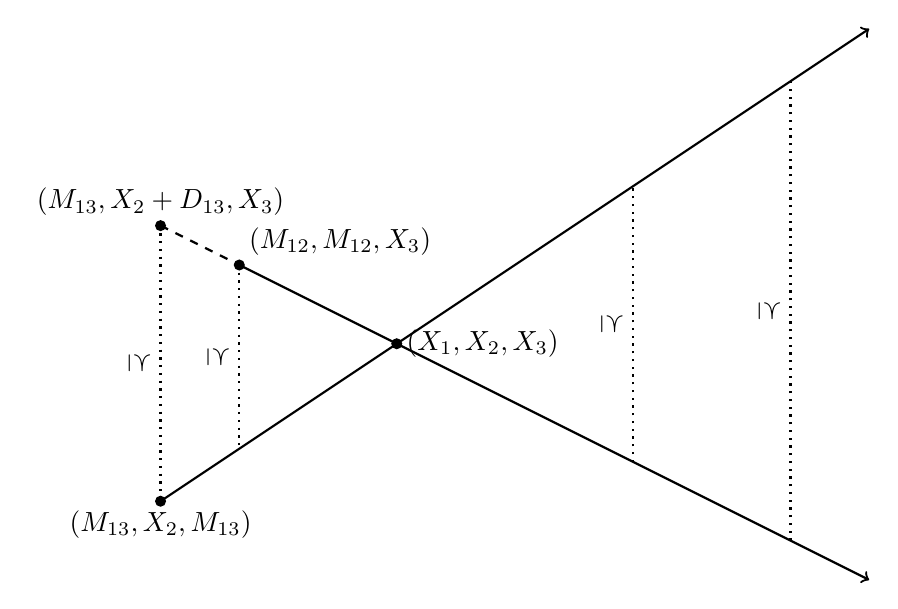
\begin{tikzpicture}
	\draw[dashed, thick] (-3, 1.5) -- (-2, 1);
	\draw[->, thick] (-2, 1) -- (6, -3);
	\draw[->, thick] (-3, -2) -- (6, 4);
	\fill (0, 0) circle(2pt) node[right] {$\left(X_1, X_2, X_3\right)$};
	\fill (-2, 1) circle(2pt) node[above right] {$\left(M_{12}, M_{12}, X_3\right)$};
	\fill (-3, -2) circle(2pt) node[below] {$\left(M_{13}, X_2, M_{13}\right)$};
	\fill (-3, 1.5) circle(2pt) node[above] {$\left(M_{13}, X_2 + D_{13}, X_3\right)$};
	\draw[dotted, thick] (-3, 1.5) -- (-3, -2) node[midway, below, rotate=-90] {$\succeq$};
	\draw[dotted, thick] (-2, 1) -- (-2, -4/3) node[midway, below, rotate=-90] {$\succeq$};
	\draw[dotted, thick] (3, -1.5) -- (3, 2) node[midway, below, rotate=-90] {$\succeq$};
	\draw[dotted, thick] (5, -2.5) -- (5, 10/3) node[midway, below, rotate=-90] {$\succeq$};
\end{tikzpicture}
\end{center}
\caption{The two $p$-values constructed corresponds to taking integrals of $g$ along these rays, that lie on a level set of $x_1 + x_2 + x_3$. The dashed line corresponds to extending the integral in the denominator of \Cref{eqn:int_extension}. The dotted lines with the majorization symbols show the majorization relation between vectors on the two rays.}
\label{fig:rays}
\end{figure}

We can re-parametrize this further, thanks to some geometric intuition (ref.\ \Cref{fig:rays}) that both $p$-values are actually integrals of $g$ along intersecting rays. We have
\begin{align}
p_{12} & = \frac{\int_0^\infty g\left(X_1 + z, X_2 - z, X_3\right) \,dz}{\int_{-D_{12}}^\infty g\left(X_1 + z, X_2 - z, X_3\right) \,dz} \nonumber \\
& \ge \frac{\int_0^\infty g\left(X_1 + z, X_2 - z, X_3\right) \,dz}{\int_{-D_{13}}^\infty g\left(X_1 + z, X_2 - z, X_3\right) \,dz} \label{eqn:int_extension} \\
p_{13} & = \frac{\int_0^\infty g\left(X_1 + z, X_2, X_3 - z\right) \,dz}{\int_{-D_{13}}^\infty g\left(X_1 + z, X_2, X_3 - z\right) \,dz} \label{eqn:p13}
\end{align}

Indeed from the second point \Cref{lma:two_properties} we have
$$\left(X_1 + z, X_2 - z, X_3\right) \succeq \left(X_1 + z, X_2, X_3 - z\right)$$
for $z \le 0$ and the majorization reversed for $z \ge 0$. So Schur-concavity shows that
$$g\left(X_1 + z, X_2 - z, X_3\right) \le g\left(X_1 + z, X_2, X_3 - z\right)$$
for $z \le 0$, and the inequality reversed for $z \ge 0$. Consequently, $p_{12} \ge p_{13}$ by comparing \Cref{eqn:int_extension,eqn:p13}.

For the alternative case where $X_2 \ge M_{13}$, it follows from a similar proof. In either cases, $p_{12} \ge p_{13}$, or in generality, $p_{12} \ge p_{1j}$ for $j \ge 1$. A test based on only $X_1$ and $X_2$ is sufficient for the null hypothesis $H_{0j}$, if the carrying measure $g$ is Schur-concave. By \Cref{thm:stoch}, rejecting this null hypothesis is equivalent to inferring that $X_1 \ge X_j$ for all $j>1$ stochastically.

\end{proof}

As the construction of this test follows \cite{Fithian:2014ws}, it is also a uniformly most powerful unbiased selective level-$\alpha$ test.

If the distribution is discrete, the proof above holds true. Instead of performing integrals, the lattice points on the rays will be summed. If ties are broken independently and randomly, as in \Cref{sec:multinomial_example}, the end points on the rays can be considered as half a point.

\section{Selective confidence bound}
\label{sec:selective_confidence_bound}

We can take the idea above further and construct confidence bound for $\theta_1 - \max_{j>1} \theta_j$. This can be achieved by considering a statistical test, to see if $\theta_1 - \max_{j>1} \theta_j \le \delta$, followed by the duality of confidence interval and statistical test.

\begin{theorem}
In the same setup as \Cref{thm:main_result}, there is a selective level-$\alpha$ lower confidence bound for $\theta_{\left(1\right)} - \max_{j>1} \theta_{\left(j\right)}$.
\end{theorem}

\begin{proof}

Again we start with assuming $X_1 \ge \cdots \ge X_n$. The null hypothesis $H_{01}^\delta$ can be thought of as $\bigcup_{j > 1} H_{0j}^\delta$, where $H_{0j}^\delta$ is $\theta_1 - \theta_j \le \delta$. In other words, we focus on the conditional law
$$\mathcal{L}_{\theta_1 - \theta_j = \delta} \left(D_{1j} \middle| D_{1j}, X_2, \ldots, X_n, A\right),$$
which is the truncated distribution
\begin{align*}
D_{1j} & \sim \exp\left(\left(\theta_1 - \theta_j\right) D_{1j} + \theta_2 X_2 + \cdots + \left(\theta_1 + \theta_j\right) M_{1j} + \cdots + \theta_n X_n \right) \\
& ~~~~~~~~ g\left(M_{ij} + D_{ij}, X_2, \ldots, M_{ij} - D_{ij}, \ldots X_n\right) 1_{A_1} \\
& \sim \exp\left(\delta D_{ij}\right) g\left(M_{ij} + D_{ij}, X_2, \ldots, M_{ij} - D_{ij}, \ldots X_n\right) 1_{A_1}.
\end{align*}

The $p$-values thus are
$$p_{1j} = \frac{\int_{D_{1j}}^\infty \exp\left(\delta z\right) g\left(M_{1j} + z, X_2, \ldots, M_{1j} - z, \ldots, X_n\right) \,dz}{\int_{\max\left\{X_2 - M_{1j}, 0\right\}}^\infty \exp\left(\delta z\right) g\left(M_{1j} + z, X_2, \ldots, M_{1j} - z, \ldots, X_n\right) \,dz}.$$

As before in \Cref{sec:exponential_families}, without loss of generality we assume $n = 3$. Once again it is sufficient to show that $p_{12} \ge p_{13}$. We have the same two cases. If $X_2 < M_{13}$, then
\begin{align*}
p_{12} & = \frac{\int_0^\infty \exp\left(\delta \left(z + D_{12}\right)\right) g\left(X_1 + z, X_2 - z, X_3\right) \,dz}{\int_{-D_{12}}^\infty \exp\left(\delta \left(z + D_{12}\right)\right) g\left(X_1 + z, X_2 - z, X_3\right) \,dz} \\
& \ge \frac{\int_0^\infty \exp\left(\delta z\right) g\left(X_1 + z, X_2 - z, X_3\right) \,dz}{\int_{-D_{13}}^\infty \exp\left(\delta z\right) g\left(X_1 + z, X_2 - z, X_3\right) \,dz} \\
p_{13} & = \frac{\int_0^\infty \exp\left(\delta \left(z + D_{13}\right)\right) g\left(X_1 + z, X_2, X_3 - z\right) \,dz}{\int_{-D_{13}}^\infty \exp\left(\delta \left(z + D_{13}\right)\right) g\left(X_1 + z, X_2, X_3 - z\right) \,dz} \\
& = \frac{\int_0^\infty \exp\left(\delta z\right) g\left(X_1 + z, X_2, X_3 - z\right) \,dz}{\int_{-D_{13}}^\infty \exp\left(\delta z\right) g\left(X_1 + z, X_2, X_3 - z\right) \,dz}
\end{align*}

The same argument in \Cref{fig:rays} shows that $p_{12} \ge p_{13}$. This is again true for the case where $X_2 \ge M_{13}$ as well. This means that the bound can be constructed considering only $p_{12}$.

\end{proof}

\section{Step down procedure}
\label{sec:step_down_procedure}

If one is interested in verifying more than just the ``winner'', this selective test can also be extended as a step-down procedure to verify the ``first runner-up'' and ``second runner-up'' etc., while controlling the FWER and the FDR.

Formally, we wish to find the biggest $j$ such that we can infer
$$\theta_1 > \ldots > \theta_j > \max_{k>j} \theta_k.$$
If $j_0$ is the true value of $j$, the two error rates we mentioned above refer to
$$\text{FWER} = \PP\left(j \ne j_0\right) ~~~~ \text{ and } ~~~~ \text{FDR} = \EE\left[\frac{\left(j - j_0\right)_+}{j}\right],$$
where $\left(j - j_0\right)_+ / j$ is taken to be $0$ if $j = 0$.

\begin{theorem}
There is a step-down procedure that infers $j_0$ above with both the FWER and FDR controlled at $\alpha$.
\end{theorem}

\begin{proof}

This can be fitted into the selective sequential model selection framework proposed by Fithian, Taylor and Tibshirani \cite{Fithian:2015uj}. Given the observations $X_1 \ge \cdots \ge X_n$, drawn from an unknown distribution $F$, we consider the sequence of null hypothesis of
$$H_{0j}: \theta_j \le \max_{k > j} \theta_k.$$
Alternatively, we can think of them as a sequence of nested model
$$M_0\left(X\right) \subseteq M_1\left(X\right) \subseteq \cdots \subseteq M_n\left(X\right), ~~~~~~~~ M_j\left(X\right)^c = \left\{\theta_1 > \cdots > \theta_j > \max_{k > j} \theta_k\right\},$$
and the each $M_j$ depends on $X$ through the order of $X$. The step-down procedure for rejecting $H_{0j}$ is equivalent to selecting the smallest $j$ for which $F \in M_j\left(X\right)$.

We can construct selective $p$-values by conditioning on $M_j\left(X\right)$, as well as other nuisance parameters. Specifically, we are conditioning on the selection of the model $M_j\left(X\right)$. We can take $p_j$ to be the survival function of the conditional law
\begin{align}
&~ \mathcal{L}_{\theta_j = \theta_{j+1}} \left(D_{j\left(j+1\right)} \middle| M_j\left(X\right), X_1, \ldots, X_{j-1}, M_{j\left(j+1\right)}, X_{j+2}, \ldots, X_n\right) \nonumber \\
= &~ \mathcal{L}_{\theta_j = \theta_{j+1}} \left(D_{j\left(j+1\right)} \middle| \left\{X_1 > \ldots > X_j > \max_{k > j} X_k\right\}, X_1, \ldots, X_{j-1}, M_{j\left(j+1\right)}, X_{j+2}, \ldots, X_n\right) \nonumber \\
= &~ \mathcal{L}_{\theta_j = \theta_{j+1}} \left(D_{j\left(j+1\right)} \middle| \left\{X_{j-1} > X_j > M_{j\left(j+1\right)}\right\}, X_1, \ldots, X_{j-1}, M_{j\left(j+1\right)}, X_{j+2}, \ldots, X_n\right). \label{eqn:step_down_law}
\end{align}

\begin{figure}[htbp]
\begin{center}
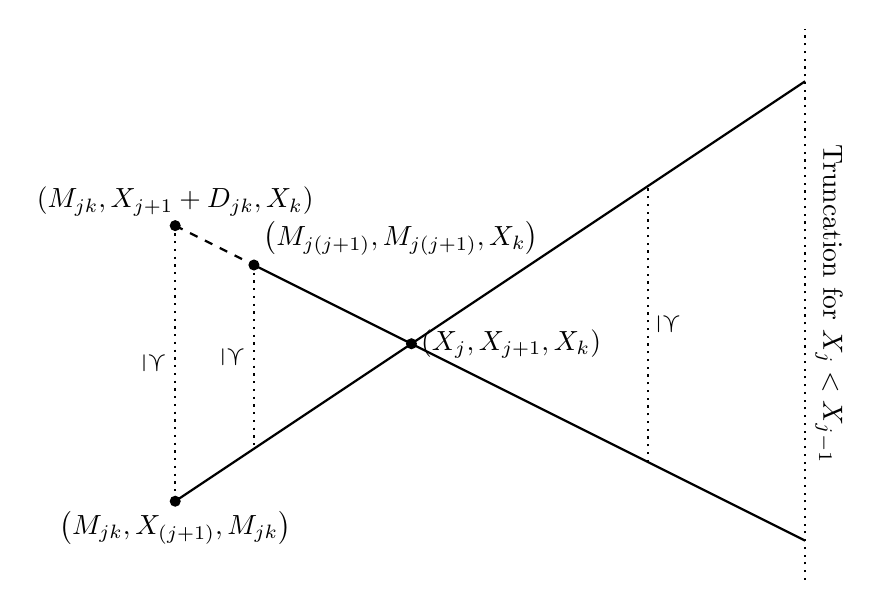
\begin{tikzpicture}
	\draw[dashed, thick] (-3, 1.5) -- (-2, 1);
	\draw[thick] (-2, 1) -- (5, -2.5);
	\draw[thick] (-3, -2) -- (5, 10/3);
	\fill (0, 0) circle(2pt) node[right] {$\left(X_j, X_{j+1}, X_k\right)$};
	\fill (-2, 1) circle(2pt) node[above right] {$\left(M_{j\left(j+1\right)}, M_{j\left(j+1\right)}, X_k\right)$};
	\fill (-3, -2) circle(2pt) node[below] {$\left(M_{jk}, X_{\left(j+1\right)}, M_{jk}\right)$};
	\fill (-3, 1.5) circle(2pt) node[above] {$\left(M_{jk}, X_{j+1} + D_{jk}, X_k\right)$};
	\draw[dotted, thick] (-3, 1.5) -- (-3, -2) node[midway, below, rotate=-90] {$\succeq$};
	\draw[dotted, thick] (-2, 1) -- (-2, -4/3) node[midway, below, rotate=-90] {$\succeq$};
	\draw[dotted, thick] (3, -1.5) -- (3, 2) node[midway, above, rotate=-90] {$\succeq$};
	\draw[dotted, thick] (5, -3) -- (5, 4) node[midway, above, rotate=-90] {Truncation for $X_j < X_{j-1}$};
\end{tikzpicture}
\end{center}
\caption{The two $p$-values constructed corresponds to taking integrals of $g$ along these segments, that lie on a level set of $x_j + x_{j+1} + x_k$. The dashed line corresponds to extending the integral in the denominator of \Cref{eqn:int_extension}. The dotted line on the far right is the truncation that enforces $X_j < X_{j-1}$.}
\label{fig:crop_rays}
\end{figure}

Here we are only comparing $X_j$ to $X_{j+1}$ by \Cref{sec:exponential_families}. The upper truncation for $X_j$ can be represented by cropping \Cref{fig:rays} along a vertical line, shown in \Cref{fig:crop_rays}, thus the proof of \Cref{thm:main_result} on sufficiency to compare $X_1$ and $X_2$ remains valid with appropriate conditioning. Again we can construct the $p$-values as in \Cref{eqn:p1j} for $k>j$.

$$p_{jk} = \frac{\int_{D_{jk}}^{X_{j-1}} g\left(X_1, \ldots, M_{jk} + z, \ldots, M_{jk} - z, \ldots, X_n\right) \,dz}{\int_{\max\left\{X_{j+1} - M_{jk}, 0\right\}}^{X_{j-1}} g\left(X_1, \ldots, M_{jk} + z, \ldots, M_{jk} - z, \ldots, X_n\right) \,dz}.$$

Hence similar to the proof of \Cref{thm:main_result}, Schur-concavity ensures $p_{j\left(j+1\right)} \ge p_{jk}$ for all $k>j$, meaning that it is sufficient to compare $X_j$ and $X_{j+1}$. In fact, we can take $p_j = p_{j\left(j+1\right)}$. These are valid selective $p$-value as required in Fithian, Taylor and Tibshirani, as
$$\PP_F \left(p_j \le \alpha \middle| M_{j-1}\left(X\right)\right) \le \alpha \text{ a.s.}, ~~~~~~~~ F \in M_{j-1}\left(X\right)$$
by tower property.

The conditioning above indeed holds some significance. The sufficient filtration \cite{Fithian:2015uj} $\mathcal{F}_k$ is given as the $\sigma$-field
\begin{align*}
\mathscr{F}_k & = \sigma\left(M_0\left(X\right), \ldots, M_j\left(X\right), X_1, \ldots, X_{j-1}, \frac{X_j + X_{j+1}}{2}, X_{j+2}, \ldots, X_n\right) \\
& = \sigma\left(\left\{X_1 > \ldots > X_j > \max_{k>j} X_k\right\}, X_1, \ldots, X_{j-1}, \frac{X_j + X_{j+1}}{2}, X_{j+2}, \ldots, X_n\right) \\
& = \sigma\left(M_j\left(X\right), X_1, \ldots, X_{j-1}, \frac{X_j + X_{j+1}}{2}, X_{j+2}, \ldots, X_n\right),
\end{align*}
which is the conditioning we used just now. Hence the nested sequence of model satisfies the subpath sufficiency principle, and the $p$-values sequence $p_j$ is independent on nulls, as defined in and shown in Theorem 4 of \cite{Fithian:2015uj}. Thus the step-down procedure where we keep rejecting $H_{0j}$ until the first time that $p_j > \alpha$ controls FWER and FDR.

\end{proof}

\section{Applications}
\label{sec:applications}

Our result above applies to a wide range of joint distributions. Note that since multiplying $-1$ preserves the majorization partial order, the following examples also work in verifying the minimum.

\begin{enumerate}

\item Correlated Gaussian: Suppose $X \sim N\left(\mu, \Sigma\right)$, where
\begin{align*}
\mu & = \left(\mu_1, \ldots, \mu_n\right), \\
\Sigma & = \begin{pmatrix}
1 & p & \cdots & p \\
p & 1 & \ddots & \vdots \\
\vdots & \ddots & \ddots & p \\
p & \cdots & p & 1
\end{pmatrix}
\end{align*}
and $p$ is fixed. Then the natural parameter is ordered the same way as $\mu$. Our test can thus be used to verify the order of the mean.

\item Multinomial distribution, e.g.\ the Iowa Republican poll example in \Cref{sec:introduction}.
$$p\left(x\right) \propto \exp\left(x^T \left(\log \pi\right)\right) \frac{1_{\left\{x_1 + \cdots + x_n = N\right\}}}{x_1! \cdots x_n!}$$
Comparing $\pi_i$ is the same $\log \pi_i$, the natural parameters. Note that the multinomial coefficient is naturally Schur-concave. The step-down procedure is applied to verify the position of the other candidates. Note that for a multinomial distribution, the conditioning \Cref{eqn:step_down_law} is equivalent to conditioning only on $M_{j\left(j+1\right)}$. We summarize the test in \Cref{tbl:poll_analysis}.

\begin{table}[htbp]
\begin{center}
\begin{tabular}{c c c c c}
\hline
Rank ($j$) & $X_{j-1}$ & $X_j$ & $X_{j+1}$ & $p$-value \\
\hline
$1$ & $\infty$ & $276$ & $214$ & $0.0065$ \\
$2$ & $276$ & $214$ & $151$ & $0.0015$ \\
$3$ & $214$ & $151$ & $71$ & $1.1126 \times 10^{-7}$ \\
$4$ & $151$ & $71$ & $36$ & $0.0014$ \\
$5$ & $71$ & $36$ & $36$ & $1.0000$ \\
\hline
\end{tabular}
\end{center}
\caption{Applying the step-down procedure to the Iowa Republican caucus. Each $p$-value is constructed by considering the conditional law in \Cref{eqn:step_down_law}, a $\text{Binomial}\left(X_j + X_{j-1}, \frac{1}{2}\right)$ truncated at $X_{j-1}$. The result was also indicated in \Cref{tbl:poll}.}
\label{tbl:poll_analysis}
\end{table}

We can also construct selective confidence bound for $\log \pi_1 - \max_{j>1} \log \pi_j$, i.e.\ find a $\delta^*$ such that
$$\PP_{H_{01}^\delta} \left(\text{reject } H_{01}^\delta: \log \pi_1 - \max_{j>1} \log \pi_j \le \delta \middle| A_1\right) < 0.05,$$
according to \Cref{sec:selective_confidence_bound}.

Once again, for multinomial distribution, conditioning on $M_{12}, X_3, \ldots, X_n$ is the same as conditioning on $M_{12}$, which gives $X_1 \sim \text{Binomial}\left(X_1 + X_2, \frac{e^\delta}{e^\delta + 1}\right)$, truncated at $M_{12}$. There is a maximum $\delta^*$ for this truncated binomial distribution has a survival function of $0.05$ at $X_1$.

This gives $\delta^* = 0.103142$. This translates to $\log \pi_1 - \max_{j>1} \log \pi_j \ge 0.103142$, or $\pi_1 / \max_{j>1} \pi_j \ge 1.10865$, with $0.95$-confidence. Or in terms of the Iowa Republican poll example, Trump has relatively around $11\%$ more support than any other candidates. This is smaller than the number deduced from raw vote count, $\left(276 - 214\right) / 214 \approx 29\%$, accounting for selection bias.

\item Independent binomials
$$p\left(x\right) \propto \exp\left(x^T \left(\log p\right)\right) \frac{1}{p_1! \left(N-p_1\right)! \cdots p_n! \left(N-p_n\right)!}$$

\item Round robin tournaments with the Bradley--Terry model, where each player has a score $\theta_i$, and the probability of player $j$ winning against player $k$ is
$$\frac{e^{\theta_j - \theta_k}}{1 + e^{\theta_j - \theta_k}} = \frac{e^{\left(\theta_j - \theta_k\right) / 2}}{e^{\left(\theta_j - \theta_k\right) / 2} + e^{\left(\theta_k - \theta_j\right) / 2}}.$$

Suppose $Y_{jk} = 1$ if $j$ beats $k$ and $Y_{jk} = 0$ if $k$ beats $j$. We will also adopt the convention that $Y_{jk} + Y_{kj} = 1$. Thus the joint distribution of $\left(Y_{jk}\right)_{j, k}$ is
$$p\left(\left(y_{jk}\right)_{j, k}\right) \propto \exp\left(\sum_j 2\theta_j \sum_{k \ne j} y_{jk}\right)  = \exp\left(\theta^T x\right),$$
where $x_j = \sum_{k \ne j} y_{jk}$. In other words, $x_j$ is the number of wins by player $j$.

If the individual results are masked and we only know about the net wins, then
$$p\left(x\right) \propto \exp\left(2\theta^T x\right) g\left(x\right),$$
where $g\left(x\right)$ is a function that count number of possible tournament results giving the net win vector $x$. A bijection proof shows that $x$ is indeed Schur-concave, allowing to apply the main result in comparing $2\theta$ and thus $\theta$.

\end{enumerate}

\bibliographystyle{plain}
\bibliography{papers,additional}

\end{document}